\documentclass[tikz,border=4pt]{standalone}
\usepackage[T1]{fontenc}
\usepackage{lmodern}
\usetikzlibrary{arrows.meta,fit,backgrounds,positioning}
\begin{document}
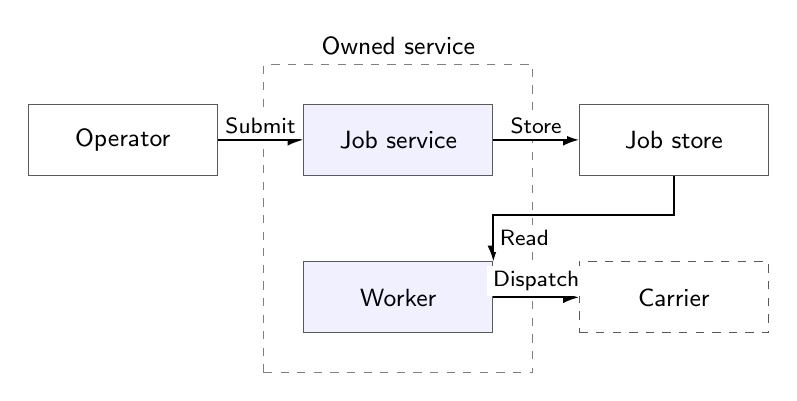
\begin{tikzpicture}[
  box/.style={draw=black!65,minimum width=24mm,minimum height=9mm,align=center,
    font=\sffamily\fontsize{9}{11}\selectfont,inner sep=3pt},
  edge/.style={-{Latex[length=2mm]},line width=.7pt},
  edge label/.style={font=\sffamily\fontsize{8.5}{10}\selectfont,fill=white,inner sep=2pt}]
  \node[box] (operator) at (0,0) {Operator};
  \node[box,fill=blue!6] (service) at (3.5,0) {Job service};
  \node[box] (store) at (7,0) {Job store};
  \node[box,fill=blue!6] (worker) at (3.5,-2) {Worker};
  \node[box,dashed] (carrier) at (7,-2) {Carrier};
  \begin{scope}[on background layer]
    \node[draw=black!50,dashed,fit=(service)(worker),inner sep=5mm,
      label={[font=\sffamily\fontsize{9}{11}\selectfont]above:Owned service}] {};
  \end{scope}
  \draw[edge] (operator) -- node[edge label,above] {Submit} (service);
  \draw[edge] (service) -- node[edge label,above] {Store} (store);
  \draw[edge] (worker) -- node[edge label,above] {Dispatch} (carrier);
  \draw[edge] (store.south) -- ++(0,-.5) -| node[edge label,pos=.75,right] {Read} (worker.north east);
\end{tikzpicture}
\end{document}
